%!TEX TS-program = pdflatex
%!TEX root = i3det-top.tex
%!TEX encoding = UTF-8 Unicode

% additional definitions
\newcommand{\degC}[1]{$\unit[#1]{^\circ{C}}$}
%\newcommand{\mA}{\mbox{\unit{mA}}}
% definition to produce a "less than or similar to" symbol
\def\lsim{\mathrel{\rlap{\raise 0.2ex\hbox{$\,<\,$}}{\lower 0.9ex\hbox{$\,\sim\,$}}}}
% definition to produce a "greater than or similar to" symbol
\def\gsim{\mathrel{\rlap{\raise 0.2ex\hbox{$\,>\,$}}{\lower 0.9ex\hbox{$\,\sim\,$}}}}


\section{\label{sec:dom}The Digital Optical Module}

\subsection{\label{sec:dom_functional} A Functional Description of the DOM}

The DOM is the fundamental light sensor and data acquisition unit for IceCube.
It consists of a spherical glass housing 
containing a downward-facing $10^{\prime\prime}$ diameter photomultiplier tube (PMT)
and associated circuit boards that allow near-autonomous operation (Figure~\ref{fig:domcomponents}) .
Data acquisition, control, calibration, communication and low voltage power conversion 
are integrated in one annular circuit board that fits around the neck of the PMT (Main Board)~\cite{ref:domdaq}. 
Separate circuit boards generate PMT high voltage, interface to the PMT pins~\cite{ref:pmt},
delay PMT signals, and generate calibration light flashes that can reach other DOMs.
Key requirements for the DOM include
the precise recording of a wide variety of PMT pulse widths and amplitudes, robustness in
a challenging deployment environment, and long term reliability.

%============================================================
\begin{figure}
\vspace{3pt}
\begin{tabular}{c@{\hspace{0pt}}c}
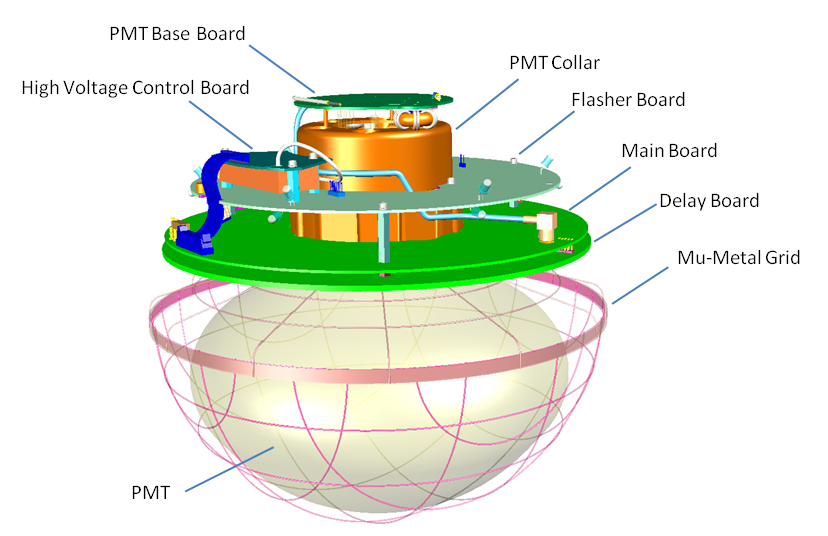
\includegraphics[width=0.49\textwidth,clip=true]{graphics/dom/functional/domfig1a-DOM3DModel.png} & \
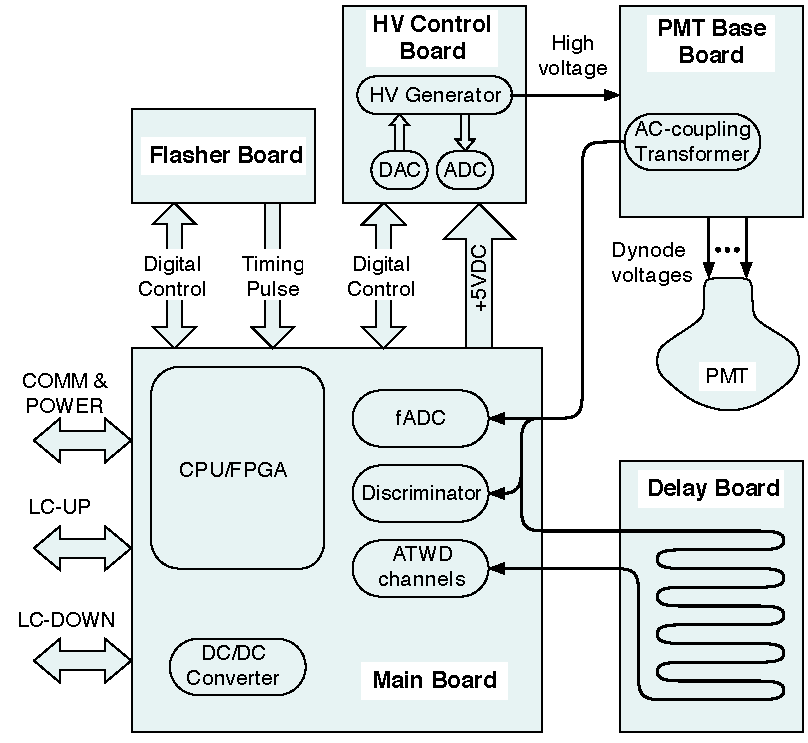
\includegraphics[width=0.49\textwidth,clip=true]{graphics/dom/functional/domfig1b-DOMBlockDiagram.pdf} \\
\end{tabular}
\caption{Components of the DOM, showing mechanical layout (left) and functional connections (right).
}
\label{fig:domcomponents}
\end{figure}
%============================================================


The PMT detects
signals from neutrino events ranging over energies \unit[10]GeV--\unit[10]PeV
and  distances  from a few meters to \unit[500]m away.
Corresponding PMT waveforms can have amplitudes from \unit[1]mV up to and beyond the linearity limit
of the PMT (\unit[$\sim2$]volts) and widths from \unit[12]nsec to \unit[1500]nsec.
In order to accommodate such a variety of signals,
the DOM includes multiple digitizers with overlapping dynamic range and different sampling speeds
(Section~\ref{sec:mainboard})~\cite{ref:domdaq}.
Each DOM is triggered independently by detection of individual photons, starting a 
recording of the PMT waveform that includes further photons arriving up to \unit[6.4]{$\mu$sec} later.
The trigger time is saved along with the
waveform shape, which reveals the times of arriving photons relative to this reference.
The DOM typically accumulates such triggered data for a period of ? to \unit[?]sec before sending as a block.
Separately, the PMT trigger rate is recorded in \unit[0.1]sec intervals,
as a collective increase of all rates could signify detection of many low energy neutrinos
in case of a Galactic supernova event (see Sec.~\ref{sec:online:supernova}).

DOMs transmit their data to computers in the IceCube Laboratory building using a twisted wire pair that also provides
power.  Wire pairs are bundled together to form the vertical down-hole cables and the horizontal surface cables.  
Each wire pair is shared between two DOMs, with data transfers initiated by a surface computer.
Separately, dedicated wiring to neighbor DOMs above and below allows 
quick recognition of local coincidences where nearest or next-to-nearest neighbors trigger within
a common \unit[1]$\mu$sec time window.
Local coincidence triggers often have complex PMT waveforms reflecting multiple photons
detected in each DOM, which are therefore
saved in full detail; otherwise the DOM saves abbreviated information appropriate to single photon
detection (Section~\ref{sec:mainboard})~\cite{ref:domdaq}.

The DOM is capable of interpreting commands from the surface that specify tasks for configuration, 
data taking and transmission, monitoring or self-calibration.
Self-calibration functions establish PMT and amplifier gains as well as sampling speed (Section~\ref{sec:domcal}).
The RAPCal system(Section~\ref{sect:dom:rapcal}) is implemented for tracking each local DOM clock's offset from universal time,
allowing PMT pulses that were independently recorded in many DOMs  to be recombined into events by surface computers.

\subsection{\label{sec:dom_components} Components}

\subsubsection{\label{sec:sphere}Glass Sphere and Harness}

The glass sphere housing has diameter $13^{\prime\prime}$ and thickness $0.5^{\prime\prime}$.  
Spheres are specified to protect the inside electronics and PMT against long term applied pressure of 
\unit[250]bar (\unit[2.6]km water depth)
as well as temporary overpressure up to \unit[690]bar during refreezing of melted ice in the drill hole.
They were produced by Benthos, Inc., based on a design for deep sea environments but using glass
with very low potassium or other radioactive trace elements that would contribute to the dark noise
count rate (Section~\ref{sect:darknoise}).  
%N.B. not borosilicate, according to analysis shown at final CDR 2005 (Claire's slides), in contrast
%to the Benthos sphere datasheet which says borosilicate
Optical transmission was measured in representative samples as 93\% at \unit[400]nm,
decreasing to 50\% at \unit[340]nm and 10\% at \unit[315]nm (normal incidence, excluding Fresnel reflection).

All spheres were tested up to \unit[10,000]psi hydrostatic pressure by the manufacturer.
Each was delivered as two hemispheres that mate precisely at the equator.
After assembly of other components into the sphere, it is evacuated and backfilled with dry nitrogen,
a butyl rubber sealant is applied around the seam, and the sealant is covered with wide plastic tape.
The interior gas pressure is set to 0.5 bar so the seal remains tight even
at ambient south pole air pressure 0.6 bar.

The DOM is held by an aluminum waistband with rubber gaskets against
the glass above and below the equator seam. 
Figure~\ref{fig:domcable} shows how it is attached to the main down-hole cable via a system
of steel rope and chain that carries the weight load around the DOM.
The main cable bends around the DOM, and the DOM axis stays vertically aligned with the string.

%============================================================
\begin{figure}
\vspace{3pt}
\begin{tabular}{c@{\hspace{0pt}}c}
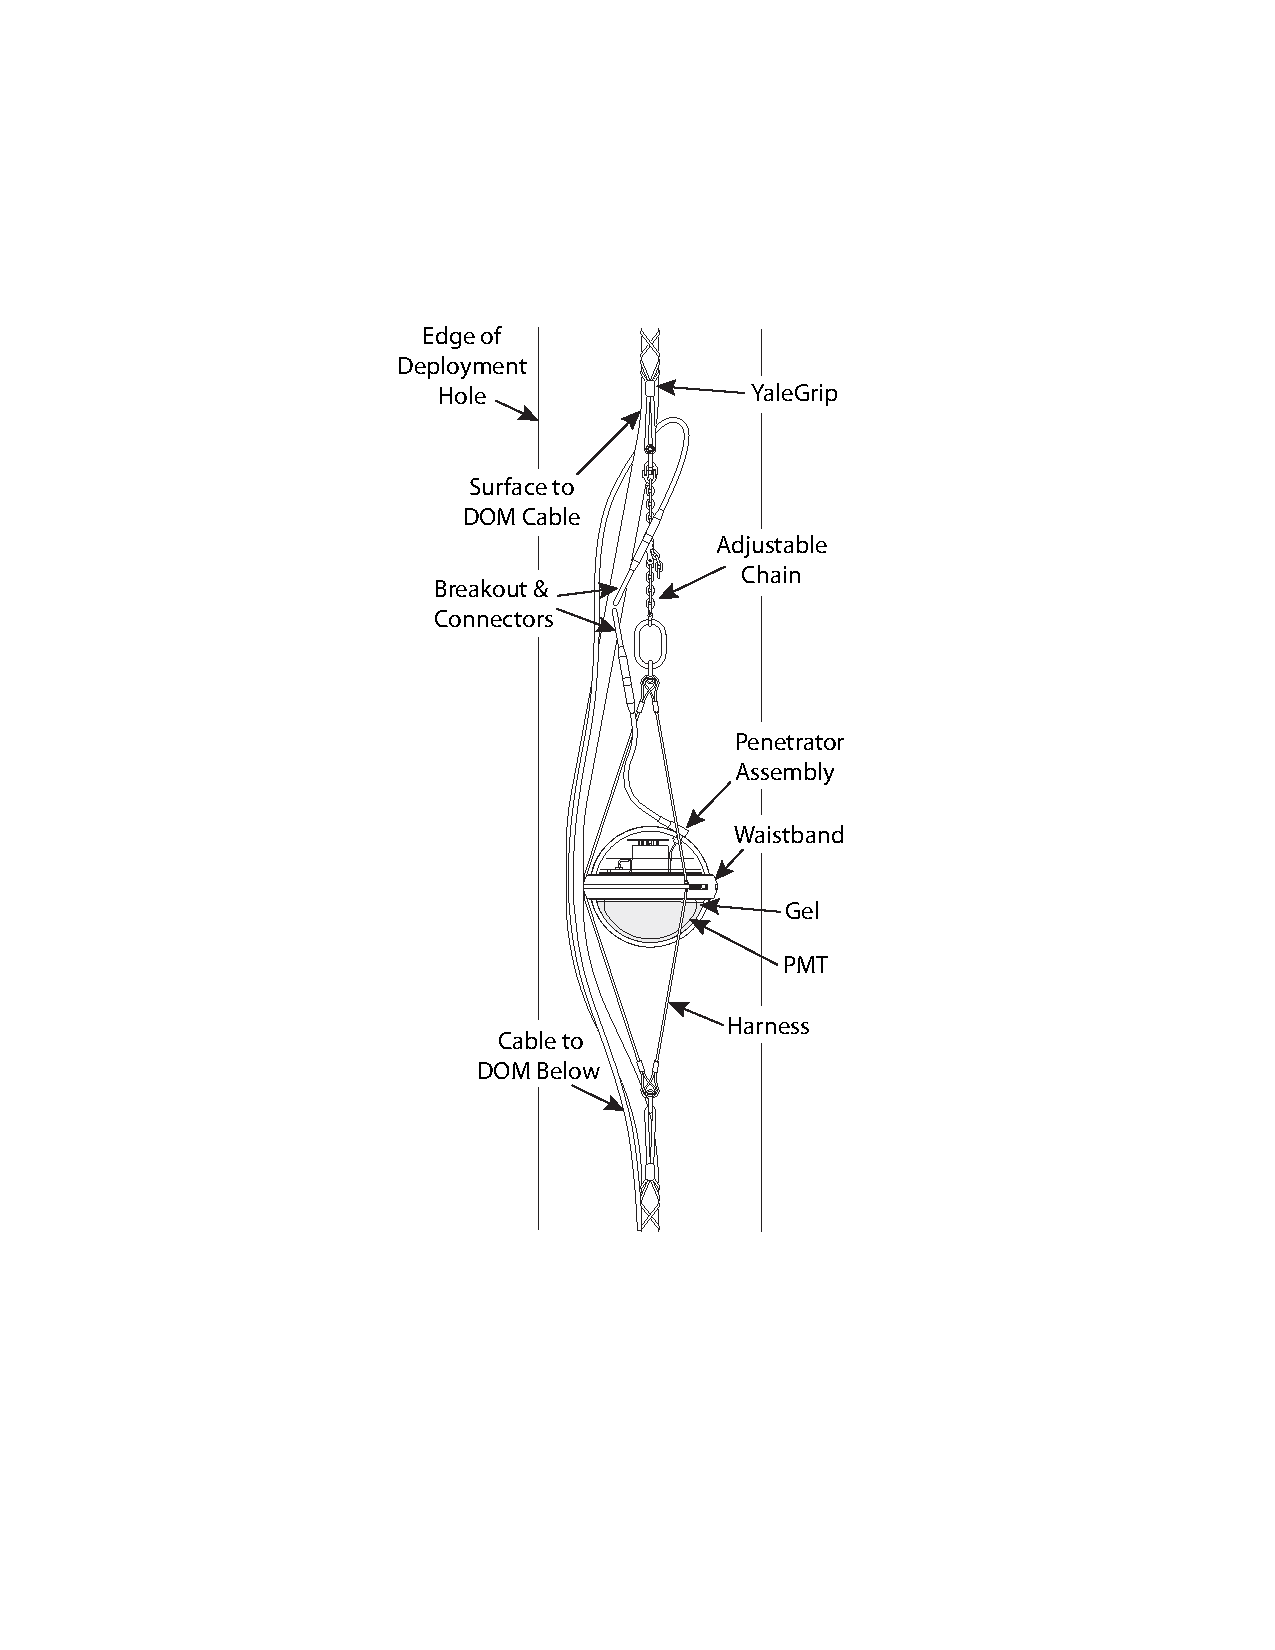
\includegraphics[width=0.49\textwidth,clip=true]{graphics/dom/functional/domfig2a-CableAssembly.pdf} & \
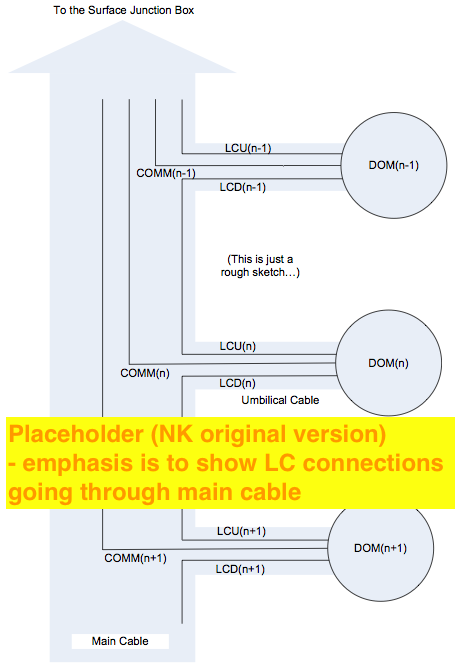
\includegraphics[width=0.49\textwidth,clip=true]{graphics/dom/functional/domfig2b-CableConnections.png} \\
\end{tabular}
\caption{FIXME Cable figure needs caption, figure to be updated
}
\label{fig:domcable}
\end{figure}
%============================================================

%NK section 3.4.1 text:
%The spherical pressure housing consists of two hemespheres made of low expansion borosilicate
%glass that seal at the equator. Each pair of mating hemespheres have been tested for pressure
%tightness at 10,000 psi (689 bar) by the manufacturer. [The pressure must operate continuously
%under 250 bar (2.6 km-deep water) and allow the over pressure of 689 bar (refreezing pressure) for
%seven days. 9400-0029-PCR.] The top hemesphere has a 16.3 mm-diameter hole for installing the
%penetrator assembly (below) that facilitates electrical connections to the interior electronics without
%compromising the pressure tightness.
%The pair of glass hemespheres consitutes more than 9 Kg of mass (9.07 Kg) and is potentially a
%significant source of photonic noise arising from the decay of radioisotope content. The IceCube
%spheres are produced with a special attention to eliminate pottasium content and minimize other
%radioactive trace elements, such as cerium. [According to Chemir Analytical Services report, June
%2005, the pottasium concentration was below the detection level and that of cerium was less than
%40 ppm by ICP analysis; however, in a separate University of Washington measurement, non-zero
%numbers are seen under pottasium. Without any write up to accompany the measurement, we
%don’t know how to interpret the numbers.] The manufacturer’s standard material contains CaCO3
%(calcite), known to have fluorescent properties, which was also eliminated [Presumably. See Kael’s
%report, November 2003]. 

\subsubsection{\label{sec:penetrator}Cable Penetrator, Cable and Connector}

%NK section 3.4.2 text:
%(This includes the external umbilical, the internal pigtail, and the connectors on either end.) Each
%DOM requires three wire-pair connections to its interior: one pair is connected to the surface DAQ
%system and carries the bidirectional communication signals and power; another two pairs provide
%local coincidence connections to the neighboring DOMs, one above and one below.
%The penetrator is an assembly of cables and electrical feedthrough that accomplishes the 
%necessary electrical connections from outside the pressure housing through its wall while maintaining the
%pressure-tightness, characteristic impedance, and signal cross-talk requirements. It consists of a
%threaded stainless steel feedthrough that achieves the pressure-tightness by means of a single
%o-ring pressed against the glass exterior and is tightened with a spring washer and a locking nut
%from inside; a pig-tail cable that connects to the DOM main board; and a custom-designed umbili-
%cal cable containing three shielded twisted-pair cables within its jacket and having a pressure-tight
%multi-pin connector that plugs into the mating connector at one of the breakouts (see below) of the
%main cable. The umbilical cable is 0.7 m long for the type U DOM and 19.2 m long for the type T
%DOM. The umbilical cable is terminated with a dissimilar connector depending on the type of the
%DOM in order to avoid a wrong connection by human error during the deployment.

A penetrator assembly brings three wire pairs out through a \unit[16.3]mm hole in
the DOM glass.  They are routed inside a customized cable, visible in Figure~\ref{fig:domcable},
and terminate at a pressure-tight, waterproof connector that mates with a similar connector
that continues each pair into the main cable.  One wire pair carries power and a
bidirectional digital communications stream, connecting ultimately with computers in the
IceCube Laboratory building (Section~\ref{sec:cablesystems}).
The other wires lead to neighbor DOMs directly above and below,
carrying local coincidence digital pulses that signify time correlated hits in nearby DOMs (Section~\ref{sec:mainboard}).

DOMs were made in two versions, where the communications wire pair was either electrically
terminated (\unit[150]$\Omega$) or unterminated inside the DOM.  This allows each wire pair from
the surface computers to communicate with two DOMs in parallel; the terminated one is deployed
\unit[17]m or \unit[10]m below the unterminated one and therefore includes a correspondingly
long penetrator assembly cable (bottom of Figure~\ref{fig:domcable}).

The entire penetrator assembly was custom designed and produced by SEACON (California).  The part that seals against
the DOM glass is similar to a hollow steel bolt, which is secured inside the DOM by a nut and spring washer and compresses
a fluorosilicone o-ring against the outside surface.  The steel part includes additional sealing around the wires that pass through it.
Outside the DOM, a plastic shell is molded around the steel and onto the cable jacket.  
External mechanical features like the penetrator are subject to large stresses during deployment and the refreezing process;
a right angle bend outside the DOM was included for robustness, based on previous experience deploying AMANDA modules.


\subsubsection{\label{sec:pmt}PMT, Gel and Magnetic Shield}

%NK text: The gel’s primary purpose is optical coupling between the sphere and the PMT; 
%however, it also serves as a mechanical shock absorber to protect
%the PMT and the electronic assemblies during the handling, transport, and deployment. All other
%components are mounted on the PMT and no components make a mechanical contact with the
%pressure housing wall, except for the pigtail cable of the penetrator.

DOMs use the $10^{\prime\prime}$ diameter Hamamatsu R7081-02 PMT, 
or the corresponding high-quantum-efficiency (HQE) version for Deep Core strings.
Its properties have been measured and described in \cite{ref:pmt}.  It is specified by Hamamatsu for
the wavelength range \unit[300]nm--\unit[650]nm, with peak quantum efficiency around 25\% (34\% for HQE)
near \unit[390]nm.  It features a box-and-line dynode chain with 10 stages, and is operated at gain $10^7$
(Section~\ref{sec:domcal}).

The PMT bulb faces downwards in the bottom glass hemisphere, secured in high-strength 
silicone gel to a depth surrounding the photocathode area.  
The gel provides mechanical support for the whole assembly of PMT and circuit boards,
as well as good optical coupling.  
Gel thickness between PMT envelope and glass sphere is approximately \unit[1]cm.  
Originally the gel was supplied as General Electric RTV6136-D1,
and later as a similar formulation from Quantum Silicones (Virginia, USA).  
It is optically clear with transmission 97\% at \unit[400]nm, 91\% at \unit[340]nm, and 65\% at \unit[300]nm
(normal incidence).  The refractive index is 1.41, yielding less than 0.1\% Fresnel reflection as light
passes from the sphere glass into the gel and then into the PMT envelope.
The characteristics of the cured gel are specified to remain stable in the temperature range $-70^\circ$C to $45^\circ$C.

To reduce effects of the ambient magnetic field (\unit[550]mG, $17^\circ$ from vertical), a mu-metal cage surrounds the PMT bulb up to
the neck join.  It was constructed as a wire mesh with typical wire spacing \unit[66]mm and
wire diameter \unit[1]mm, blocking about 4\% of the incident light.
Without such a shield, this type of PMT would exhibit 5-10\% lower collection efficiency as well
as poorer peak-to-valley ratio and gain variations of 20\% depending on 
azimuthal orientation~\cite{calvo}.
With the shield in place, the interior magnetic field is a factor 2.8 below
the external field, pointing mostly along the axis and therefore reducing efficiency by
less than 2\% for this type of PMT.

Other interior DOM components are held in place by attachment to the PMT, mostly via screws into
a molded plastic collar glued around the neck.  The PMT base board is soldered directly to the pins.

\subsubsection{\label{sec:hv}HV Supply and Divider}

The PMT high voltage subsystem consists of a resistive voltage divider circuit (PMT Base) directly
solder-mounted on the PMT and a separate high voltage control board. 
The high voltage control board includes a DAC and an ADC for setting and reading out the PMT high voltage,
connected to the Main Board with a digital interface.  It also holds the high voltage generator, which
is a custom encapsulated module designed by EMCO (California).  The maximum high voltage is
\unit[2047]volts, specified for up to \unit[30]$\mu A$ current.  The set voltage is proportional to the DAC
output, and the actual voltage is monitored via a high-impedance divider and the ADC.  The output ripple
is less than \unit[1]mV, and stability is better than \unit[200]ppm over 8~hours.  Power consumption is
\unit[300?]mW at full load.

The generator output is carried to the PMT Base Board via a high voltage coaxial cable.  This board is
described in \cite{ICECUBE:PMT}.  Its voltage divider presents a total resistive load of \unit[130]M$\Omega$.
The PMT is operated with cathode at ground potential, so the anode signal output is AC coupled using 
a 1:1 bifilar wound toroid transformer mounted on the Base Board.
The transformer secondary is then wired to the Main Board analog input with a coaxial cable.
The single photoelectron (SPE) output waveform has been described in reference~\cite{ICECUBE:PMT}.  
With a \unit[100]$\Omega$ load connected to the transformer,  and operating at standard gain $10^7$, the SPE 
peak voltage is close to \unit[8]mV
with a FWHM \unit[7-8]nsec.  When measured on the Main Board, several effects combine to increase
the FWHM of digitized SPE waveforms to $\sim$\unit[13]nsec (peak $\sim$\unit[5]mV).

%NK section 3.5.3 text:
%The high-voltage subsystem consisits of a resistive voltage divider circuit (PMT base board) directly
%solder-mounted on the PMT and a separate high-voltage control board, consisting of a modular
%high-voltage generator and a digital interface to the main board, which provides a +5 V DC power,
%issues the on/off command, sets the high voltage output by controlling the DAC, and monitors the
%precisely scaled down value of the high voltage output by reading the ADC. The output of the
%high-voltage generator is delivered to the PMT base board by way of a high-voltage coaxial cable
%(a “pig tail” cable) originating from inside the high voltage generator. The high-voltage generator
%is modular in the sense that all the high voltage circuitry is encapsulated in this unit. Having no
%high voltage nodes exposed to anywhere other than the PMT base board allows all the failure
%mechanisms inherent to high voltage circuitry to be completely isolated within the high voltage
%generator module and the PMT base board.
%(a) PMT Base Board The design of the PMT base board in relation to the performance of the
%PMT has been already discussed in some detail in our earlier paper[3]. Here, we outline only the
%salient features. The PMT base board has been designed to minimize the power consumption while
%meeting all the performance requirements. The base board supports 1 kHz of coninuous noise
%pulses and large (explain) isolated transient pulses lasting as long as 1 us. The total resistance is
%130 MΩ, which corresponds to the maximum bleeder current of 15 ?A and the power dissipation
%of less than 30 mW. The divider ratios have been optimized for the optimum operation (maximum
%collection efficiency) of the PMT when operated at the nominal gain of 107; since the PMT has a
%manufacturing spread, this corresponds to the anode voltage of 1050 to 1600 V. Since the PMT
%operates with the cathode at ground potential (for unknown historical reasons), the PMT pulse
%signals are ac-coupled from the high anode potential to the analog front-end of the main board,
%where the digitization takes places. The ac-coupling is accomplished using a custom-designed
%1:1 bifilar-wound toroidal transformer mounted on the PMT base board. Transformer-coupling is
%reliable and virtually noise-free for our purposes unlike capacitive-coupling.
%For reliability, the circuit has been implemented using through-hole components as much as pos-
%sible, except for several low-voltage nodes where a smaller low-inductance components are pre-
%ferred. The circuit has been designed to ensure that no component is under more than 50% of the
%its rated voltage. In order to eliminate the possibility of a corona discharge, all the through-hole
%solder joints have been shaped as a smooth ”dome” by a specially-developed manufacturing tech-
%nique involving two passes of wave-soldering process (Maybe Pensar’s permission is needed to
%disclose this?).
%(b) High Voltage Generator and Control Board The high voltage generator receives a +5 V
%DC power from the main board and generates a high voltage of up to 2047 V. It has been custom-
%designed[6] for low-power, low-noise, and high reliability. The proprietary circuit consists of a quasi-
%sine oscillator running at a few 100 kHz, whose output is transformer-coupled to a diode rectifier
%circuit, low-pass filtered, and fed back to the oscillator. (This description is based on the block
%diagram of the CA Series product datasheet from EMCO website[7]. The IceCube high-votage
%generator is a customized version of this series of products.) The circuit is potted inside a steel
%case and the high voltage output exits the unit via a “pig tail” cable that reaches the PMT base
%board. The unit is compact (7 x 2.8 x 1.4 cm3) and weighs about 60 grams. The output voltage of
%the generator has a very low ripple on the order of 1 mV (spec’ed as less than 2.4 ppm, DC to 20
%MHz) and is very stable (spec: 200 ppm variations over 8 h; maybe there are actual data showing
%the stability?). The unit can source up to 30 ?A of continuous current and dissipates less than 300
%mW of power under a full power operation. The unit is capable of starting up from a cold soak
%(non-operating storage) at -55°C.

\subsubsection{\label{sec:mainboard}Main Board and Delay Board}
The Main Board and its operation has been described in detail in \cite{ref:domdaq}.  
It interfaces to other boards as shown in
Figure~\ref{fig:domcomponents} and itself provides many key functions of the DOM:

%text from NK section 3.5.1
\begin{itemize}
\item{Control all the devices inside the DOM, including the high voltage power supply for the PMT, 
the flasher board, and various sensors (pressure, temperature, power supply voltage monitor). 
Also supply necessary DC power to the subsystems.}
\item{Digitize the PMT waveforms, using the custom ASIC (ATWD: analog transient waveform digitizer) and a continuous sampling ADC.}
\item{Carry out computing functions. This includes executing PMT gain calibration, compressing 
the digitized waveform, temporarily storing the data, creating data packets and time stamping them.}
\item{Communicate with the data acquisition system on the surface.}
\item{Exchange timing pulses with the surface DAQ to calibrate the internal DOM clock. }
\item{Exchange ”local coincidence” pulses with the adjacent DOMs.}
\end{itemize}

The data flow starting from the PMT is shown in Figure~\ref{fig:domdataflow}.
PMT waveforms are amplified and compared to the discriminator threshold of \unit[0.25]SPE,
which is sufficient to begin a "launch" of the high speed waveform capture and digitization.
The \unit[300]Msps 
ATWD chips operate by analog storage of waveform samples in switched capacitor arrays of depth 128,
followed by digitization.  In order to record the waveform starting from before the discriminator
threshold crossing, the signal is first routed through the Delay Board.  Here a total delay of about
\unit[75]nsec is accomplished by a \unit[$\sim10$]m long, \unit[0.25]mm
wide, serpentine copper trace embedded in the dielectric and sandwiched between ground planes.
ATWD chips are provided with three different preamplifier gains in order to completely cover the
dynamic range of the PMT output (up to 150mA when saturated).  The highest gain channel is used
for most pulses, and lower gain recordings are also retained as needed when pulses reach within 75\% of the range 
of a higher gain channel.
As explained in Ref.~\cite{ref:domdaq}, two sets of ATWD chips are operated alternately in order to
reduce deadtime to negligible levels.

The ATWD recording interval is \unit[427]nsec.  This is ideal for reconstructing light produced within ~\unit[50]m of
a DOM, but photons from further away may arrive over a broader time interval.  Such far away signals are
also weaker, and the information is well captured in the \unit[40]Msps ADC.  This ADC samples continuously and
the FPGA is programmed to save an interval of \unit[6.4]$\mu$sec after the launch. Its preamplifier gives a dynamic 
range comparable to the high gain ATWD channel, but has extra pulse shaping to accommodate the lower
sampling speed.

Every digitizer launch results in a hit record being sent to the surface computers, but the amount of
information included depends on whether a signal was also detected in one of the neighboring DOMs.
In case of an isolated signal (no coincidence), only a time stamp and brief charge summary is sent, and
the full digitization process is aborted.  Conversely, when a nearest or next-nearest neighbor DOM 
also signals a launch within $\pm$\unit[1]$\mu$sec (local coincidence), the full waveform is compressed
and included in the hit record.  The local coincidence signaling proceeds via digital pulse codes sent on
the extra wire pairs described in Section~\ref{sec:penetrator}.
 
\begin{figure}[h]
 \centering
 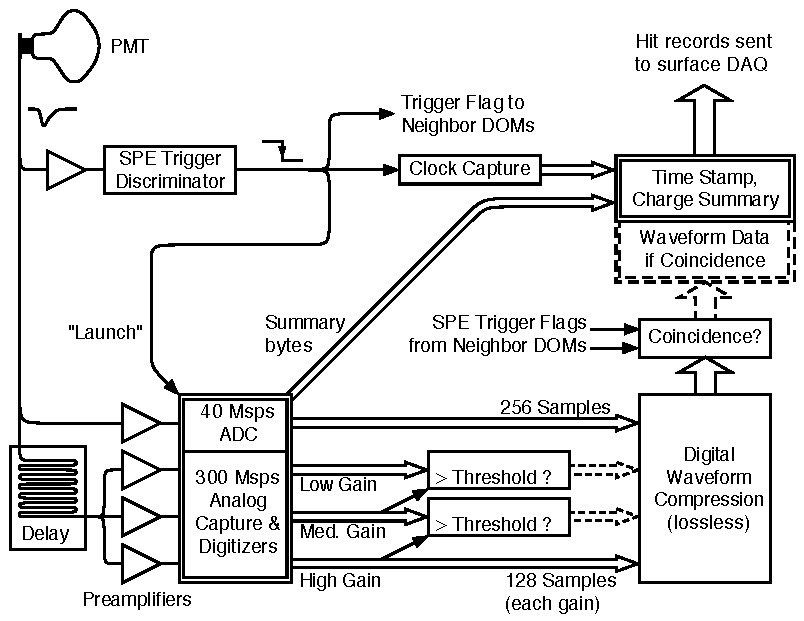
\includegraphics[width=0.6\textwidth]{graphics/dom/functional/domfig3-DOMDataFlow.pdf}
 \caption{FIXME - dom data flow needs a caption, figure may be updated}
 \label{fig:domdataflow}
\end{figure}

%NK section 3.5.2 text:
%Although low-power and high-speed, the ATWDs must be initiated by a trigger signal in order to start
%the digitizing operation. In order to capture the front pedestal of the waveform, the PMT signal is
%split in two ways: one branch enters the trigger circuit and initiates the ATWD and the other branch
%enters the delay line and emerges in the analog input of the digitizer after ?75 ns. The delay line
%is a stripline implemented as a ?10 m-long, 0.25 mm-wide, serpentine copper trace embedded in
%the dielectric and sandwiched between ground planes of the delay board. Unlike a coaxial cable
%delay line, the delay board is compact and easy to integrate into the limited space in the DOM
%sphere: the board is 3.2 mm thick and has the same area profile as the main board, below which
%it is mounted.
%(The impedance is 95 Ω. The delay time is 75±2 ns. The risetime and falltime is typically 3 ns
%(Including the source profile. ERD, Fig. 2). The signal attenuation is required to be less than 12\%.
%%The trace width was measured from ther gerber file. The trace length is based on the delay of
%0.166 ns per inch, found in the simulation file found on docushare, Document-6600.)

%%%%%%%%%%%%%%%%%%%%%%%%%%%%%%%%%%%%%%%%%%%%%%%%%%%%%%
%%[Below is more text that is too much detail for this paper]
%Several features are included for calibration functions of the DOM, also used for self-test.
%Each DOM has a local clock driven from a high-stability \unit[20]MHz(?) oscillator, in terms of which all local
%times are measured.  In order to determine slowly drifting offsets between clocks in each DOM and a master
%surface clock, the DOM provides waveform digitization of a regular timing pulse sent from the surface, as 
%well as sending a return pulse (Section~{sec:rapcal})~\cite{ref:domdaq}.
%For calibration of the waveform digitizers, the DOM has a pulser circuit that can inject programmed amounts of
%charge into the front end circuitry, and has an input multiplexer that allows the (adjustable) sampling rate
%to be calibrated via the clock oscillator.  
%A pulsed LED facilitates calibration of gain and time delay in the PMT as a function of applied high voltage 
%(Section~{sec:domcal}).

%During the first \unit[427]nsec recording interval, information is captured in one of two analog transient 
%waveform digitizers (ATWDs)
%with sampling period \unit[3.3]nsec, single bit resolution \unit[0.1?]mV for small signals and dynamic range
%\unit[7?]volts.  This period encompasses the time
%spread of most photons arriving from up to \unit[100]m away. 
%An analog delay line causes the recording to include a pretrigger period of at least \unit[10]nsec,
%allowing the leading edge to be measured with \unit[1]nsec resolution.
%For multi-photon pulses, the full arrival time profile can be reconstructed by fitting the waveform 
%as a sum of single photon responses, each contribution having typical amplitude
%\unit[5]mV and width \unit[12]nsec FWHM.
%The upper end of the dynamic range accommodates the full
%linear response range of the PMT, up to about 400(?) photoelectrons per \unit[15]nsec\cite{ref:pmtpaper}, 
%as well as fully saturated PMT pulses around \unit[5]volts amplitude.

%While the ATWDs are optimized for multi-photon events that are close to the DOM, the information
%content is more than needed for single isolated photon detections far away from the interaction,
%which may also be spread over a longer time period.
%Accordingly, the FADC is a separate 10-bit digitizer that records PMT waveforms for up to 
%\unit[6.4]{$\mu$sec} but with coarser sampling interval \unit[25]nsec.  
%This channel includes an anti-aliasing filter to broaden
%individual photon responses to \unit[70?]nsec FWHM and peak amplitude \unit[1]mV.
%With amplitude resolution \unit[0.1]mV, photon arrival times can still be determined to within \unit[7?]nsec.

%In order to quickly identify close-by events requiring full ATWD information, the cabling system includes
%extra wiring for DOMs to communicate directly with neighbors above and below~\cite{ref:domdaq}.  
%Each DOM trigger can 
%thus be quickly classified by whether a nearest or next-to-nearest neighbor DOM also
%triggered within a \unit[$\pm$1]$\mu$sec time window.  Such a local coincidence causes the full length
%ATWD and FADC waveforms to be saved, and otherwise only three FADC samples are saved along with
%the reference timestamp.
%%[End of text that is too much detail for this paper]
%%%%%%%%%%%%%%%%%%%%%%%%%%%%%%%%%%%%%%%%%%%%%%%%%%%%%%





\subsubsection{\label{sec:flasher}Flasher Board}
%NK section 3.5.4 has extensive description and simplified diagram

Each IceCube DOM contains a flasher board. The standard IceCube
flasher board, which is included in every DOM except the color DOMs
described below, is a circular board fitted with 12 LEDs (ETG-5UV405-30) with a peak
wavelength of 399~nm; the FWHM of the LED spectrum is
14~nm. The LEDs are arranged in pairs, evenly spaced around the board
with a 60$^{\circ}$ separation between each pair. One LED in each pair
points outward horizontally, the other LED is tilted upward at an angle
of 48$^{\circ}$, which is close to the Cherenkov angle in ice (n =
1.36). The angular emission profile of each LED has a FWHM of
30$^{\circ}$ in air, which is modeled as a Gaussian emission profile
with $\sigma = 13^{\circ}$. After refraction through the DOM glass and into
the ice, the value of $\sigma$ is 9.7$^{\circ}$ in the polar direction
and 9.8$^{\circ}$ in the azimuthal direction for the tilted LEDs, and  9.2$^{\circ}$ in the polar direction
and 10.1$^{\circ}$ in the azimuthal direction for the horizontal LEDs.

The LEDs are controlled by a current pulse applied to each LED through
a high speed MOSFET driver with a series resistor. The LEDs can be turned on individually or in any
combination of the 12, using a bitmask in the flasher DAQ
configuration. The photon output of the LED depends on the width and
brightness, or
amplitude of
the driving current pulse. The current amplitude is controlled by the
brightness setting in the flasher DAQ, which may have a value between
0 and 127; the maximum LED
current is 240~mA. The current pulse width is controlled by the width
setting in the flasher DAQ, which is twice the current pulse width in
nanoseconds and may have a value between 0 and 127; the maximum current pulse width is 70~ns. The
minimum stable pulse width that we can achieve is about 6~ns. The
photon output is related to the brightness  and width by the following
empirically derived relationship:
\begin{equation}
N = 1.17 \times 10^{10} \left (0.0006753 + 0.00005593B \right ) \left
  (W + 13.9 - \frac{57.5}{1 + B/34.4} \right )
\end{equation}
where N is the number of photons, B is the brightness setting (maximum
value 127) and W is the width setting (maximum value 127). The photon
output per LED ranges from $10^6$ to $10^{10}$ photons per flash,
which is equivalent to the energy output of GeV - 100 TeV cascades. The maximum
LED pulse rate is 610~Hz. The current waveform is read out by ATWD
digitizer channel~3 during flasher operation in order to measure the
precise rise time of the flasher pulse. The flasher light output
begins 8.3~ns after the current pulse is recorded. Although flashers can be
operated in multiple DOMs in the same run, the DAQ does not support
time-synced flashing of LEDs on different DOMs, so coincident flasher
events happen only by chance. 

The flasher LEDs are used for a variety of calibration purposes:
\begin{itemize}
\item verifying the timing response of the DOMs throughout the
  software
\item measuring the position of the deployed DOMs in ice
\item measuring the optical properties of the ice
\item verifying the performance of cascade reconstruction algorithms
  in measuring position, direction and energy
\end{itemize}

{\it Color DOMs}

There are 16~DOMs (8 on string~79 in the center of IceCube, 8 on
string~14 on the edge of IceCube) fitted with multiwavelength flasher boards, called
color DOMs or cDOMs. Each cDOM includes 3 LEDs with a nominal
wavelength of 505~nm, 3 LEDs with a nominal wavelength of 450~nm, 3
LEDs with a nominal wavelength of 370~nm and 3 LEDs with a nominal
wavelength of 340~nm. The LEDs are arranged in pairs as on the
standard flasher board, but all LEDs point outward horizontally. The
arrangement of the pairs is shown in Figure XXcdom sketch from cdom
wikiXX. The properties of the LEDs are given in
Table~\ref{table:cdom_properties}.

\begin{table}
\caption{Properties of the cDOM LEDs, including wavelength $\lambda$ and
  angular emission FWHM $\sigma$.}
\begin{tabularx}{\linewidth}{|c|c|c|c|X|X|X|}
  \hline
 LED& nominal $\lambda$ & measured $\lambda$ & $\sigma$ air & $\sigma$
 DOM, polar & $\sigma$ DOM, azimuthal \\
\hline
UVTOP335-FW-TO39 &340 nm&338 nm&	51.0$^{\circ}$ &	36.1$^{\circ}$ &	42.9$^{\circ}$\\
\hline
NS370L\_5RFS &370 nm&	371 nm&55.2$^{\circ}$&	39.1$^{\circ}$&	42.9$^{\circ}$\\
\hline
LED450-01 & 450 nm& 447 nm&	6.8$^{\circ}$ &	4.8$^{\circ}$ &	5.3$^{\circ}$ \\
\hline
B5-433-B505 & 505 nm& 494 nm& 6.4$^{\circ}$ &	4.5$^{\circ}$ 	&4.9$^{\circ}$ \\
\hline
\end{tabularx}
\label{table:cdom_properties}
\end{table}

\subsection{\label{sec:dom_prodtest}  Production and Testing}

DOM Integration and Test had some clear objectives as the IceCube project
moved from the instrumentation design stage to the production and
installation at the Pole phase of the project’s construction. One,
approximately 5500 in-ice and IceTop DOMs were required to be built, tested
and delivered to the South Pole. Two, all of the DOMs must meet the
stringent quality requirements needed for them to work reliably buried deep
in the ice for more than 20 years of lifetime. Finally, this work must be
done such that the DOMs were delivered on time, within budget and that they
meet all technical specifications. The IceCube project’s principal
bottleneck for delivering science was the hot water drilling to be done
each austral summer at the South Pole. It was critically important that
drilling never stopped on account of an instrumentation inventory shortage
of any kind. The instrumentation needed to deploy into each successfully
drilled hole to be ready. This dictated a DOM Production strategy that was
based on electronics manufacturing best practices and a team that was
committed to success. Additional challenges included lack of electronics
manufacturing infrastructure within the IceCube Collaboration, multi-site
production, cultural differences, South Pole logistics chain and an
unpredictable project funding profile. The DOM Production plan was
implemented in a 3-stage approach. Stage 1 was to produce 400 DOMs at the 3
DOM production sites. This was a sufficient quantity to supply
instrumentation for the 1st year drilling plan of 4 holes at Pole and to
verify DOM production readiness at all locations. It also allowed for the
DOM design to be verified as good after a deployment season. If major
design problems were discovered, they could be addressed before significant
material supplies were purchased. Stage 2 was the procurement of materials
and supplies for another 1000 DOMs. Lastly, the last stage procurements
were done for the remaining 4100 DOMs to be integrated and tested.

The planning stage for DOM Production was when the manufacturing
infrastructure was installed at the 3 DOM Production sites. It was
organized in 5 areas of focus: Methodology, Materials, Labor, Equipment,
and Environment. Methodology referred to the actual process flow to
integrate and test a DOM. The process flow was required to be fixed so it
could be successfully transferred to each site. A DOM Process Traveler was
created which listed each process step required. In addition, the date,
technician and material serial numbers were recorded onto the Process
Traveler. All the information was then entered into a central DOM
Production database. Each DOM was to be individually tested and its data
reviewed by someone independent of the production team prior to shipment to
Pole. Materials required for DOM integration and test was listed in the
controlled document called Bill of Materials. Sole source procurements were
identified early and executed. Suppliers were actively managed during DOM
Production with regular visits to the vendor sites. It was expected that
all materials were fully tested at the supplier sites and were delivered to
the DOM production sites Certificates of Conformance indicating that the
materials were acceptable for use in the DOM production environment. Some
materials, such as the PMT and sphere, were directly drop shipped to the
DOM production sites. Everything else was shipped to the US DOM production
site (Physical Sciences Laboratory (PSL), Stoughton, Wisconsin) where they
were kitted for delivery to the 2 European DOM Production sites (DESY,
Zeuthen, Germany and Stockholm University, Sweden). Discrepant materials
discovered during the manufacturing process were segregated and
dispositioned accordingly via a rigorous Quality Control system. Total
material purchases were made so that the ending material inventory was very
small. The intent was for all materials to be converted into working
DOMs. Labor was planned at each site for continuous DOM production. All
technicians were trained and certified to perform integration and test
tasks. Each site had separate Quality function personnel. Equipment used
for DOM integration and test was the same at all sites. It was either made
custom per specified drawings at each site or was made at PSL and shipped
to DESY and Stockholm University for use. All jigs were qualified for use
prior to introduction in the manufacturing process. Measurement equipment
was calibrated and records maintained that verified their traceability to a
reference standard. DOM integration took place in an ESD, temperature and
humidity controlled environment. Separate areas were established for
inventory storage, Work in Process (WIP), non-conforming materials and
finished DOMs ready to ship. Each integration site was kept very clean to
minimize the introduction of contaminants that might result in failed
components. Finally, each of the 3 DOM production sites had to be qualified
for production by passing a rigorous inspection. In summary, the
introduction of manufacturing protocols based on electronics industry best
practices allowed for each site to be independent yet produce DOMs that
were form, fit and function identical. Weekly phone calls each week between
the sites tracked progress and performance. 

The actual DOM integration and test process was composed of 18 discrete
steps tracked via the Process Traveler. The first 15 steps related to
integration while the last steps were concerned with Final Acceptance
Testing (FAT), DOM harness attachment and final packing procedures needed
before shipping to the South Pole. The integration process started with the
PMT Collar attachment to the PMT. The PMT Collar provided a mounting point
for the electronic boards needed inside a DOM. The PMT was then mounted
into a special jig that allowed for precise placement inside the bottom
glass hemisphere. In parallel, the mu metal shield  was placed inside the
bottom hemisphere and a silicone dielectric gel was mixed and poured into
the same hemisphere. The gel was then degassed. After degassing, the PMT
was placed in the gel and it was allowed to cure for 48 hours before
further processing. After curing, the PMT High Voltage Base was soldered
onto the flying leads of the PMT. Separately, the PC Board stack was made
by attaching the Delay Board, Main Board, Flasher Board and High Voltage
Control Board together with screws and standoffs. After PC Board stack
assembly, it was mounted onto the PMT collar and attached with 3 small
screws. The penetrator assembly was mounted into the top hemisphere and the
two halves of the sphere were brought together so the penetd functionality
was confirmed to be good before the DOM moved to Final Acceptance Testing
(FAT).

All DOMs at all sites were required to pass a rigorous testing protocol at
cold temperatures in a dark environment before shipping to the South
Pole. The testing was done in Dark Freezer Labs (DFLs) that were maintained
at each production site. In addition to acceptance testing, individual DOM
characterization was done to inform future physics analyses. The main
functional test was called the Simple Test Framework (STF) which was a
self-diagnostic functional test installed on each Main Board. DOM
Calibration (DOMCal) was also performed along with local coincidence
testing. The tests were done at various temperatures during the typical 22
days in the DFL (see Fig.~\ref{fig:fat_cycle}). A key element in FAT was to compare testing
results at the beginning of the testing with those attained at the final
room temperature test. Major changes in parameters were flagged as
potential problems and were dispositioned accordingly. Approximately xx
performance parameters were evaluated and measured during FAT. The typical
first pass rate for DOMs during FAT was approximately 90\% (check
this). After the successful completion of FAT, DOM deployment harnesses
were attached and the DOMs individually packed in custom cartons that were
then combined into overcartons that held 8 DOMs ready for shipment. DOMs
were additionally tested on the ice at the South Pole prior to deployment
into the ice. This was done to ensure DOMs did not sustain any damage as a
result of a strenuous journey to Pole. Eight overcartons were placed on a
custom sled that allowed for testing of 64 DOMs at a time. They were
covered with an additional cover that helped block any light from reaching
the DOMs in their packaging. STF testing was done along with a measurement
of dark rates before final installation into the holes. Of the
approximately 5500 DOMs shipped to Pole, about 30 were shipped back to the
US after failing on-ice testing.    

\begin{figure}[!h]
 \centering
 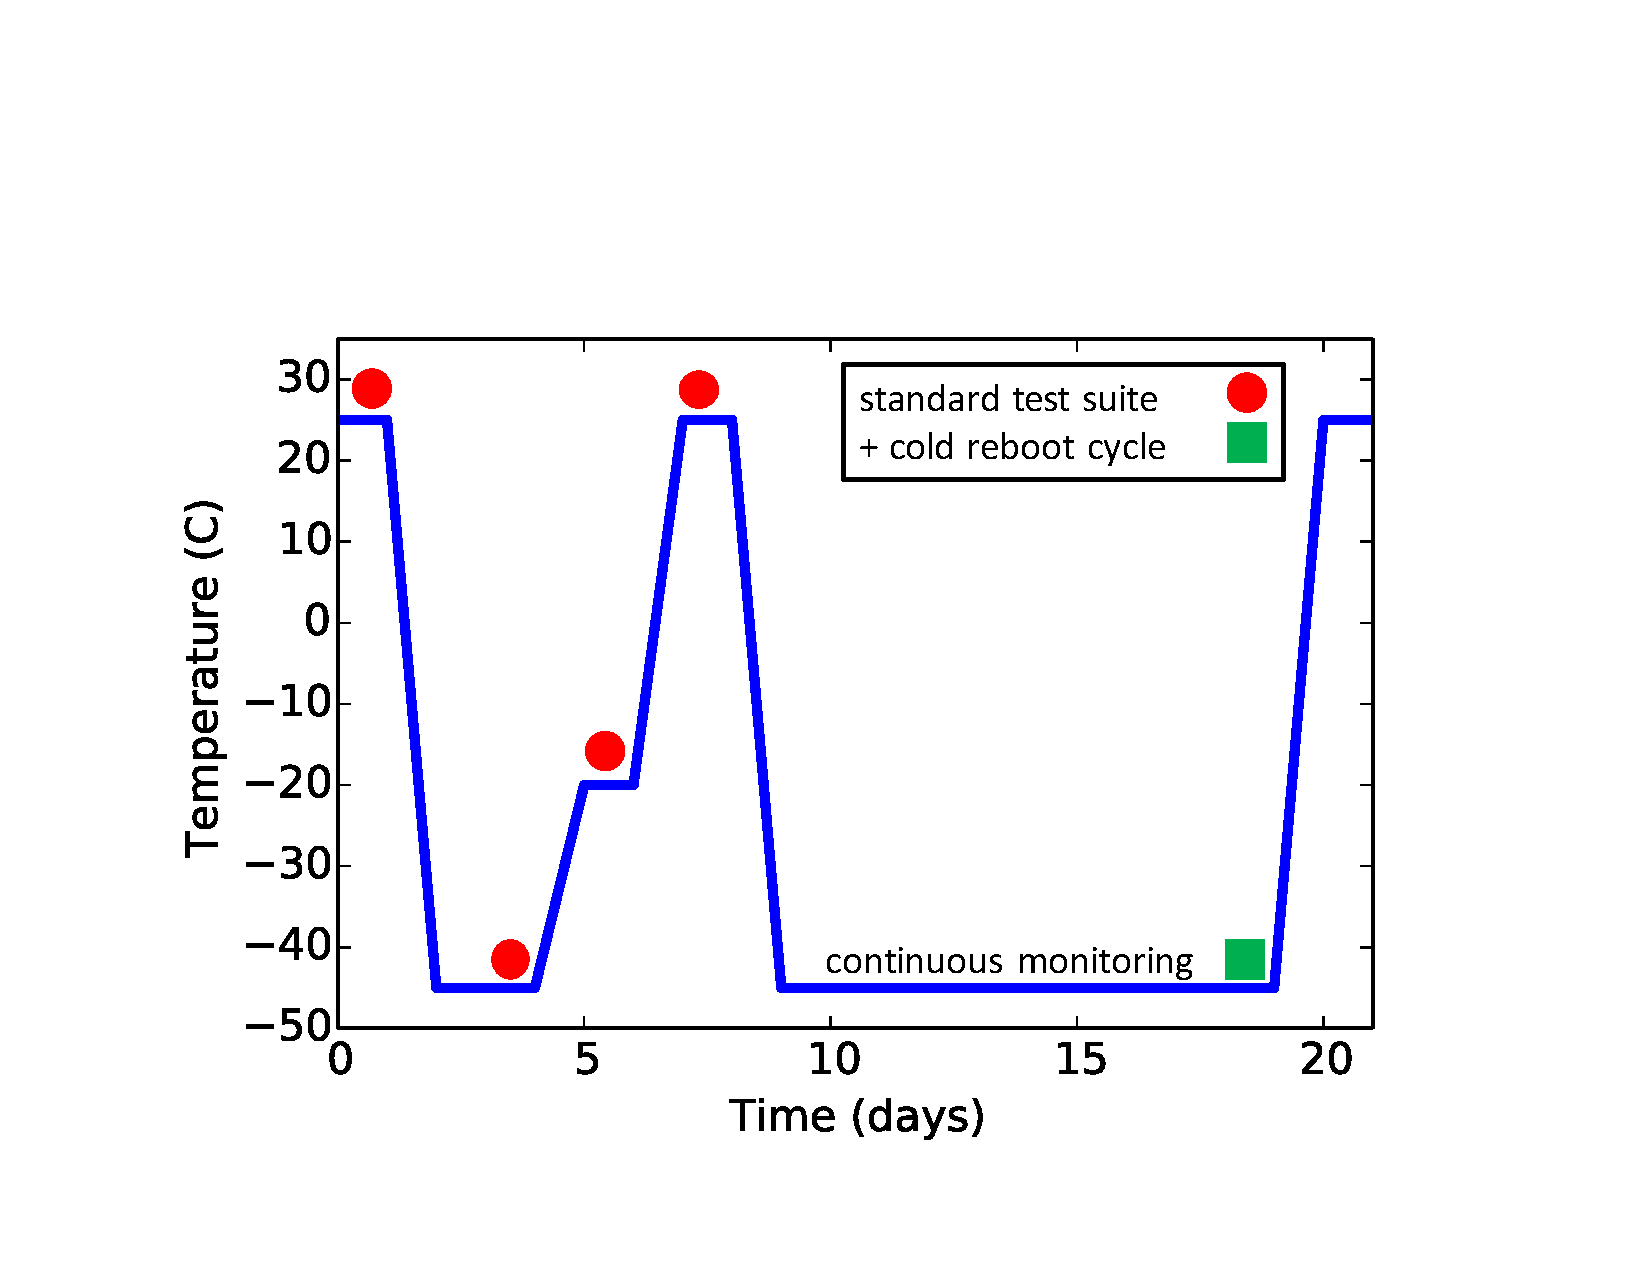
\includegraphics[width=0.9\textwidth]{graphics/dom/production/fat_cycle.pdf}
 \caption{Final Acceptance Test (FAT) temperature profile, including
   testing steps performed at each stage.}
 \label{fig:fat_cycle}
\end{figure}

\subsection{\label{sec:reliability}Reliability}

As the DOMs are not serviceable after deployment, an extensive testing
protocol including temperature-cycling and cold-soaking ensured that bad
modules and early component failures were identified before shipping.
All DOMs were also re-tested at the South Pole before final deployment, to
screen out any modules damaged during transit.

As of 2016, 5397 of the 5484 deployed DOMs ($98.4\%$) are operating in
data-taking mode in the data acquisition system (see Table
\ref{tab:dom_failures}).  We classify DOM 
failures into two broad categories: failures during deployment and
freeze-in, and failures during subsequent operation.  The majority of the
failures (55) occurred before post-deployment commissioning; we hypothesize
that these are primarily attributable to cable failures, water leaks,
or freeze-in damage. 32 DOMs have failed after commissioning, and
we include in this count modules on a wire pair taken out of service when
the partner DOM on the same pair failed.  No particular pattern in the
failures is observed, other than they are typically during non-standard
operation or an exceptional event: a power outage, calibration run, or
flash filesystem upgrade.  The most recent two DOMs failed on May 23, 2013,
losing communications after a power outage.  Diagnosis of DOM failures
beyond identifying electrical shorts is challenging.

A number of DOMs have developed issues that affect their data-taking
configuration but are still usable.  The local coincidence settings of DOMs of
functional DOMs adjacent on a string to dead DOMs must also be
modified. These are enumerated in Table \ref{tab:dom_failures}.  

\begin{table}[h]
  \centering
  \caption{Number of DOM failures during deployment/freeze-in and after
    commissioning during detector operation, as well as DOMs with various
    issues (including a failed neighbor) causing them to be operated in a
    non-standard data-taking mode.} 
  \label{tab:dom_failures}
  \begin{tabular}{| r | c |}
    \hline
    \bf{DOM failures} & \bf{87} \\
    \hline    
    deployment / freeze-in & 55 \\
    post-commissioning & 32 \\
    \hline
    \hline
    \bf{DOMs in Non-standard Mode} & \bf{171} \\
    \hline
    bad digitizer & 12 \\
    reduced PMT gain & 1 \\
    non-standard local coincidence & 158 \\
    \hline    
  \end{tabular}
\end{table}

We can estimate the surviving fraction of DOMs 25 years after the original
deployment, assuming a constant, random failure rate after freeze-in.
Specifically, we calculate the Wilson score binomial confidence interval of
survival probability using the post-commissioning failure rate of DOMs
\cite{Wilson_Score}.  The estimated survival fraction as a function of
time is shown in Fig.~\ref{fig:dom_survival}; currently we estimate the
surviving fractEion in 2030 to be $97.3\pm0.3\%$.  While this simplified
model does not account for an increase in failure rate due to component aging, the
observed failure rate since detector completion of $2.0~\mathrm{yr}^{-1}$ is
significantly lower than the mean predicted rate of $4.5~\mathrm{yr}^{-1}$.  We attribute
this to infant mortality and/or to improved operational protocols that
minimize the number of DOM power cycles.

\begin{figure}[!h]
 \centering
 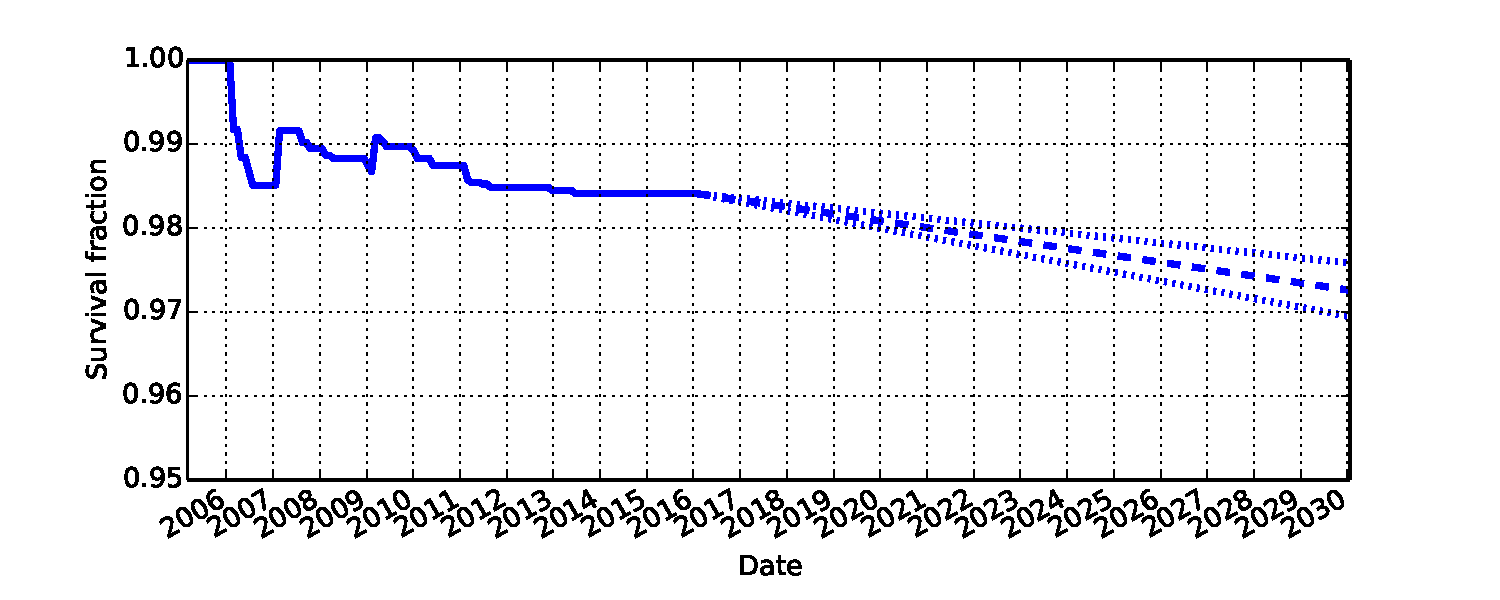
\includegraphics[width=0.95\textwidth]{graphics/dom/reliability/dom_survival.pdf}
 \caption{Actual and predicted fraction of surviving DOMs versus time, based on an assumed
 constant post-freeze-in failure rate.  The dotted lines indicate the
 central and 95\% CL estimates.  Increases before 2011 are due
 to deployments of new strings.} 
 \label{fig:dom_survival}
\end{figure}
